\subsection{Unassessed exercise 3}
\subsubsection{Question 11: ER modelling}
Develop (extended) entity-relationship diagrams (complete with multiplicities and annotations) to model the following real-world situations:

\begin{enumerate}[label=\alph*.]
    \item A tourist information system is to provide information about tourist attractions in British cities. For each city, the system must know about the county the city is located in. Attractions must include at least all major parks, museums, and theatres. For each attraction the system must be able to provide information about the street it is located in. It should also know about other main streets, how long they are, and which intersects with which.
    \item A database is required to provide information about hotels, bed and breakfast places, and youth hostels. It should be possible to query it for the nearest airport or for any tourist attractions in the vicinity. In case a place is fully booked, the system could be used to find alternative accommodation nearby. The system should be aware of different types of room, such as ``single'', ``double'', etc., and typically a house will have rooms of more than one category (and its rates will depend on the category). Hotels may offer conference facilities in the form of meeting rooms. The system should be able to list those together with their capacity and daily hiring fee.
\end{enumerate}

\begin{center}
\begin{figure}[htp]
  \centering
  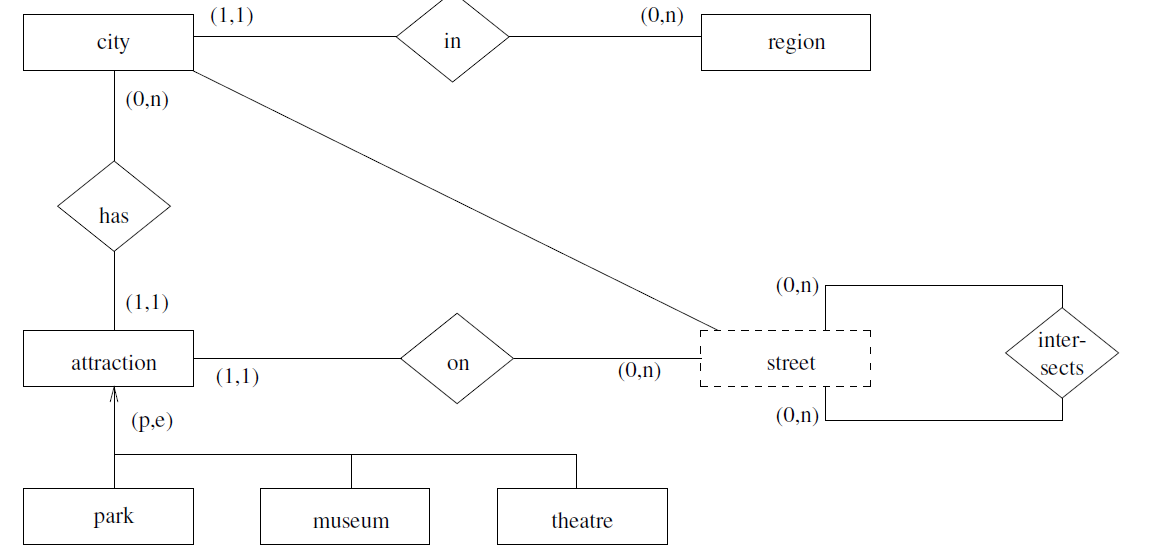
\includegraphics[width=15cm]{unit-11/figures/01.png}
%   \caption*{The structure of a packet frame.}
\end{figure}
\end{center}

Note that “street” is a weak entity, depending on its containing “city” for its identity. This is natural because
we do not expect that streets have names that are unique across the whole world (or even a whole country), but are
unique within a city. (In a big city like Birmingham or London, we might need to treat each neighbourhood as a
city as well.)
The three subclasses of “attraction” are modelled using a class hierarchy. The annotations say that the subclasses
partially cover the whole class (because there can be other kinds of attractions, e.g., a historical or archaelogical
site), but the three subclasses are mutually exclusive.

% \usetikzlibrary{positioning, shapes.geometric, arrows.meta}

% \begin{center}
% \begin{tikzpicture}[
%   entity/.style={rectangle, draw, minimum width=12mm, minimum height=8mm},
%   weakentity/.style={rectangle, draw, dashed, minimum width=12mm, minimum height=8mm},
%   relationship/.style={diamond, draw, aspect=2, inner sep=1pt},
%   isa/.style={rectangle, draw=none},
%   every node/.style={font=\small},
%   node distance=15mm and 22mm
% ]

% % Entities
% \node[entity] (city) {city};
% \node[entity, right=of city] (region) {region};
% \node[entity, below=of city] (attraction) {attraction};
% \node[weakentity, right=of attraction] (street) {street};
% \node[entity, below left=of attraction, xshift=-1cm] (park) {park};
% \node[entity, below=of attraction] (museum) {museum};
% \node[entity, below right=of attraction, xshift=1cm] (theatre) {theatre};

% % Relationships
% \node[relationship, above right=6mm and 6mm of city] (in) {in};
% \node[relationship, midway, left=of attraction, xshift=-8mm] (has) {has};
% \node[relationship, midway, right=of attraction, xshift=8mm] (on) {on};
% \node[relationship, right=of street, xshift=12mm] (intersects) {intersects};

% % Connections
% \draw (city) -- node[above left] {(1,1)} (in);
% \draw (region) -- node[above right] {(0,n)} (in);

% \draw (city) -- node[left] {(0,n)} (has);
% \draw (has) -- node[left] {(1,1)} (attraction);

% \draw (attraction) -- node[below] {(1,1)} (on);
% \draw (on) -- node[below] {(0,n)} (street);

% \draw (street) -- node[above] {(0,n)} (intersects);
% \draw (intersects) -- ++(0,-1.2) node[right] {(0,n)} -| (street);

% % ISA hierarchy
% \draw (attraction) -- +(0,-7mm) |- (park);
% \draw (attraction) -- +(0,-7mm) |- (museum);
% \draw (attraction) -- +(0,-7mm) |- (theatre);

% % ISA label
% \node[isa, below=3mm of attraction] {(p,e)};

% \end{tikzpicture}
% \end{center}


\begin{center}
\begin{figure}[htp]
  \centering
  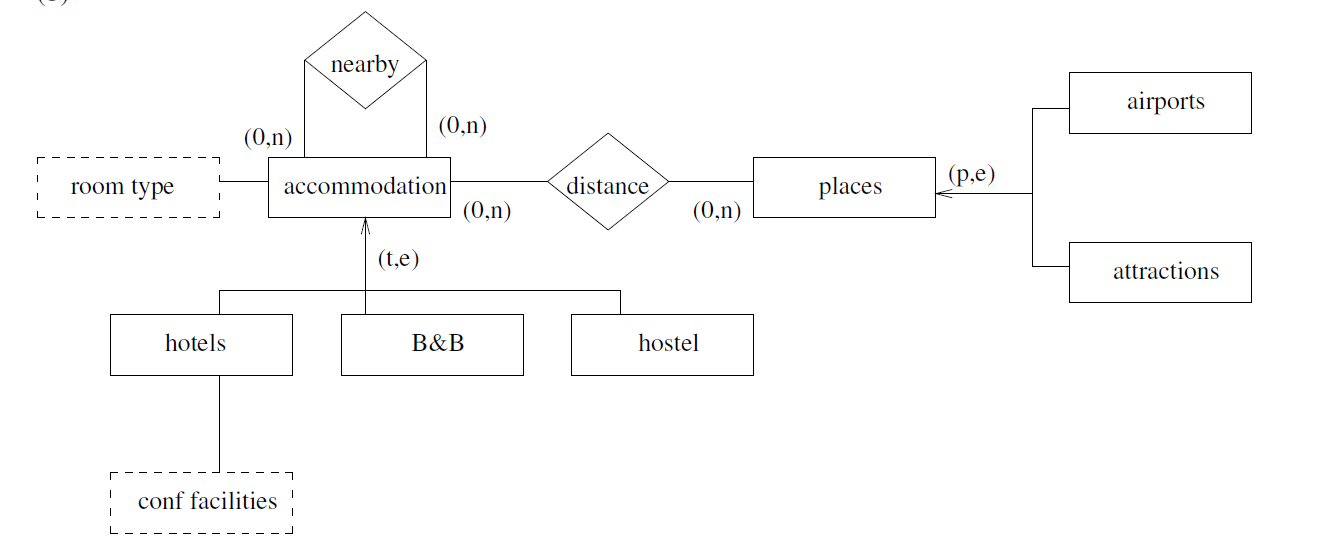
\includegraphics[width=15cm]{unit-11/figures/02.png}
%   \caption*{The structure of a packet frame.}
\end{figure}
\end{center}

\subsubsection{Question 12: ER Modeling}

Develop (extended) entity-relationship diagrams (complete with multiplicities and annotations) to model the following situations.

\begin{enumerate}[label=\alph*.]
    \item The vehicles of a car rental business fall into one of the following four classes: ``economy'', ``standard'', ``luxury'', and ``van'' (others could be added in the future). The daily rental rate is the same for all vehicles in a given class. Customers choose a class and are assigned a specific vehicle from that class by staff members. If necessary, a higher-value vehicle may substitute for a lower-value class. Besides private persons there are also commercial customers. Depending on past usage and other factors, these are granted a certain level of discount. Every commercial customer must register the employees that are eligible to take out a rental contract on behalf of the firm. The database, at this stage, does not need to deal with payments for rental agreements.

    \item An information system is to be implemented for the United Nations, to help officers retrieve information about countries. Besides obvious aspects of countries, such as populations size, capital, area, etc., the system should know about major alliances that the country is a member of. These alliances could be of military, economic, political or of a mixed nature. The system should know which continent each country is located in and which country borders against which. It should also contain information about major ethnic groups and the percentage of the population they make up. Apart from sovereign
     countries, the system should also provide the same type of information about dependent
territories and currently occupied countries. In these two latter cases the system should
know the controlling country.
\end{enumerate}

\begin{center}
\begin{figure}
  \centering
  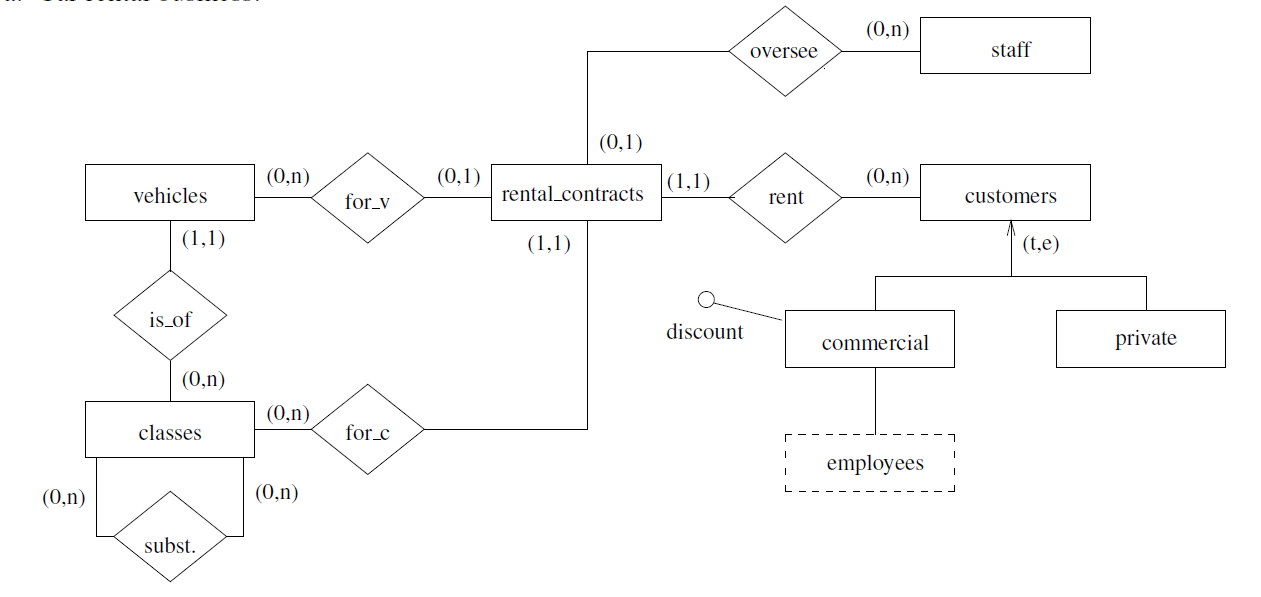
\includegraphics[width=15cm]{unit-11/figures/03.png}
%   \caption*{The structure of a packet frame.}
\end{figure}
\end{center}


\begin{center}
\begin{figure}
  \centering
  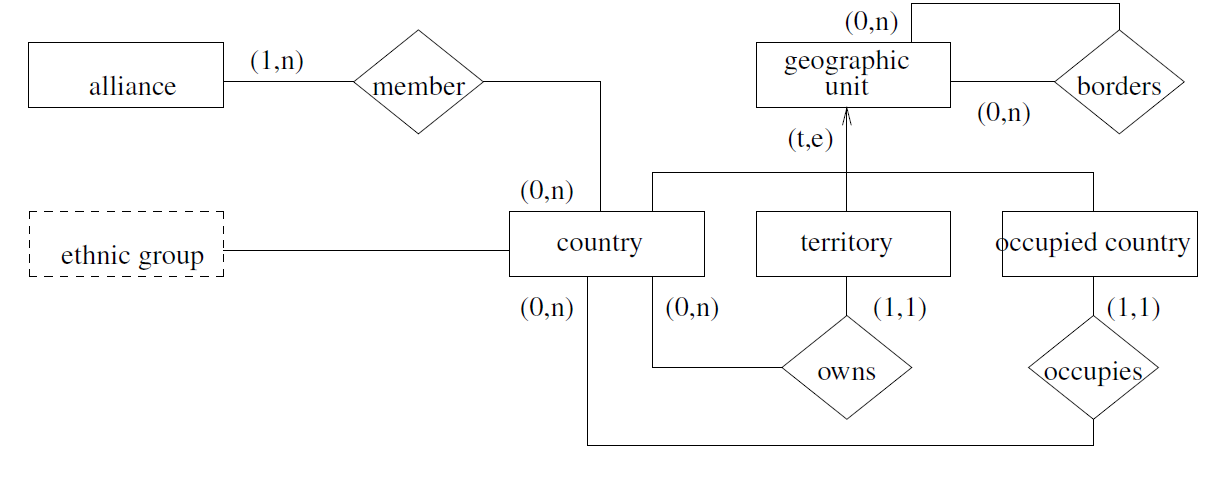
\includegraphics[width=18cm]{unit-11/figures/04.png}
%   \caption*{The structure of a packet frame.}
\end{figure}
\end{center}
% \end{document}
\subsubsection{Question 13: Logical design}

Carry out logical design (table design) for the ER-models developed for Question 11.

\begin{itemize}
    \item First define relational table schemas for all your tables using the notation:
    
    \[
    \text{table}(\underline{\text{column}_1},\ \underline{\text{column}_2},\ \ldots,\ \text{column}_i^{\circ},\ \ldots,\ \text{column}_n)
    \]
    
    Underline all the columns that make up the primary key. Use the $\circ$ superscript for columns that may be null.
    
    \item Secondly, translate the schemas into SQL \texttt{CREATE} statements. You should make sure that all the primary keys and foreign keys are declared. You should also specify the \texttt{ON DELETE} action for all the foreign keys. Feel free to add any additional constraints that seem important.
    
    Focus, in particular, on any tables for weak entities and relationships, because these tables would have foreign keys.
\end{itemize}

\subsection*{Question 14: Logical design}

Carry out logical design (table design) for the ER-models developed for Question 12. But you might omit writing \texttt{CREATE TABLE} statements if you find them tedious.
